\documentclass[10pt,a4paper]{article}
\usepackage[utf8]{inputenc}
\usepackage[T1]{fontenc}
\usepackage{amsmath}
\usepackage{amsfonts}
\usepackage{amssymb}
\usepackage{graphicx}
\usepackage{listings}
\usepackage{float}
\usepackage{subcaption}
\usepackage[labelformat=parens,labelsep=quad,skip=3pt]{caption}

\begin{document}
	\title{Homework 1 - Basic Nios Setup}
	\makeatletter
	
	\author{Zackary McClamma\thanks{University of Dayton}
		\thanks{Dept. of Electrical and Computer
			Engineering, University of Dayton, 300 College Park, Dayton, OH
			45469-0226, U.S.A. E-mail:
			mcclammaz1@udayton.edu}}
	
	\makeatother
	
	\date{\today}
	
	\maketitle
	
	\section{Introduction}
	This homework assignment involved configuring the NIOS II processor in the QuartusPrime software, adding peripherals(7 Segment Display and Buttons), and creating software to manipulate the peripherals. It being the first homework assignment the main goals were to familiarize myself with the hardware/software development process and the IDE. I was able to successfully configure the processor and create software to accomplish the tasks outlined in the assignment which were to fist display 0-9 on one of the 7 segment displays and, second to poll the state of one of the buttons on the board. In this assignment I learned how to load the processor the the FPGA, how to add inputs/outputs to the system, and how to write and execute software on the board. The rest of this document includes a description of the system, a description of how the system operates, the results from running the system, and finally in the appendices the source code for the project.
	\section{System Description}
	The system consists of three interfaces (Button, 7 Segment Display, and USB Blaster) and the CPU. The USB blaster is used to upload all of the development done in Quartus (VHDL) and Eclipse (C code) to the FPGA. The FPGA uses the VHDL code to generate the processor, memory, and also connect all the peripherals defined in the VHDL code. The C code is loaded into memory where it is read by the processor and the code is executed. This process is defined in \ref{block} below. In the figure the blue arrows indicate VHDL code, the red arrows indicate C code, and the green arrows indicate that both VHDL and C are being transmitted.  
	\begin{figure}[H]
		\centering\includegraphics[width=15cm]{HW1_Block.png}
		\caption{Embedded System Block Diagram}
		\label{block}
	\end{figure}
	\section{Theory of Operation}
	This system has one input (Button) and a set of outputs (7 Segment Display). The button uses a simple polling operation, the software runs in a loop and every iteration checks the status of the button. If the button has not been depressed "Button=1" is displayed in the console, if the button is depressed the console will display "Button=0", see Figure \ref{fig:polling}. In regards to the 7 segment display there are 7 individual LEDs within the display, each one has a corresponding memory address associated with it. If there is a 1 written to a given address the corresponding LED will be off, if a 0 is written to the address the corresponding LED is turned on. In the software there is an endless loop with a counter that counts from 0 to 9. Every time the counter is incremented the display changes to show the value the counter is at i.e. if the counter is at 3 the seven segment display will show '3'. This is achieved by writing 0 to the memory addresses that turn the segments in the display on, for example if the counter were to read 8 it would write a 0 to all of the addresses for the display. Refer to Figure \ref{fig:disp} to see the result of running the seven segment display. It should also be noted that there is approximately a 1sec. delay between display changes which is done by counting up to a large number in a for loop. The program will continuously poll the state of the button and display 0-9 on the counter until the program is terminated by the user.
	\section{Results}
	\subsection{7 Segment Display}
		\begin{figure}[H]
			\begin{subfigure}{3cm}
				\rotatebox[origin=c]{180}{\centering\includegraphics[width=3cm]{Display0.jpg}}
				\caption{Display 0}
			\end{subfigure}
			\begin{subfigure}{3cm}
				\rotatebox[origin=c]{180}{\centering\includegraphics[width=3cm]{Display1.jpg}}
				\caption{Display 1}
			\end{subfigure}
			\begin{subfigure}{3cm}
				\rotatebox[origin=c]{180}{\centering\includegraphics[width=3cm]{Display2.jpg}}
				\caption{Display 2}
			\end{subfigure}
		
			\begin{subfigure}{3cm}
				\rotatebox[origin=c]{180}{\centering\includegraphics[width=3cm]{Display3.jpg}}
				\caption{Display 3}
			\end{subfigure}
			\begin{subfigure}{3cm}
				\rotatebox[origin=c]{180}{\centering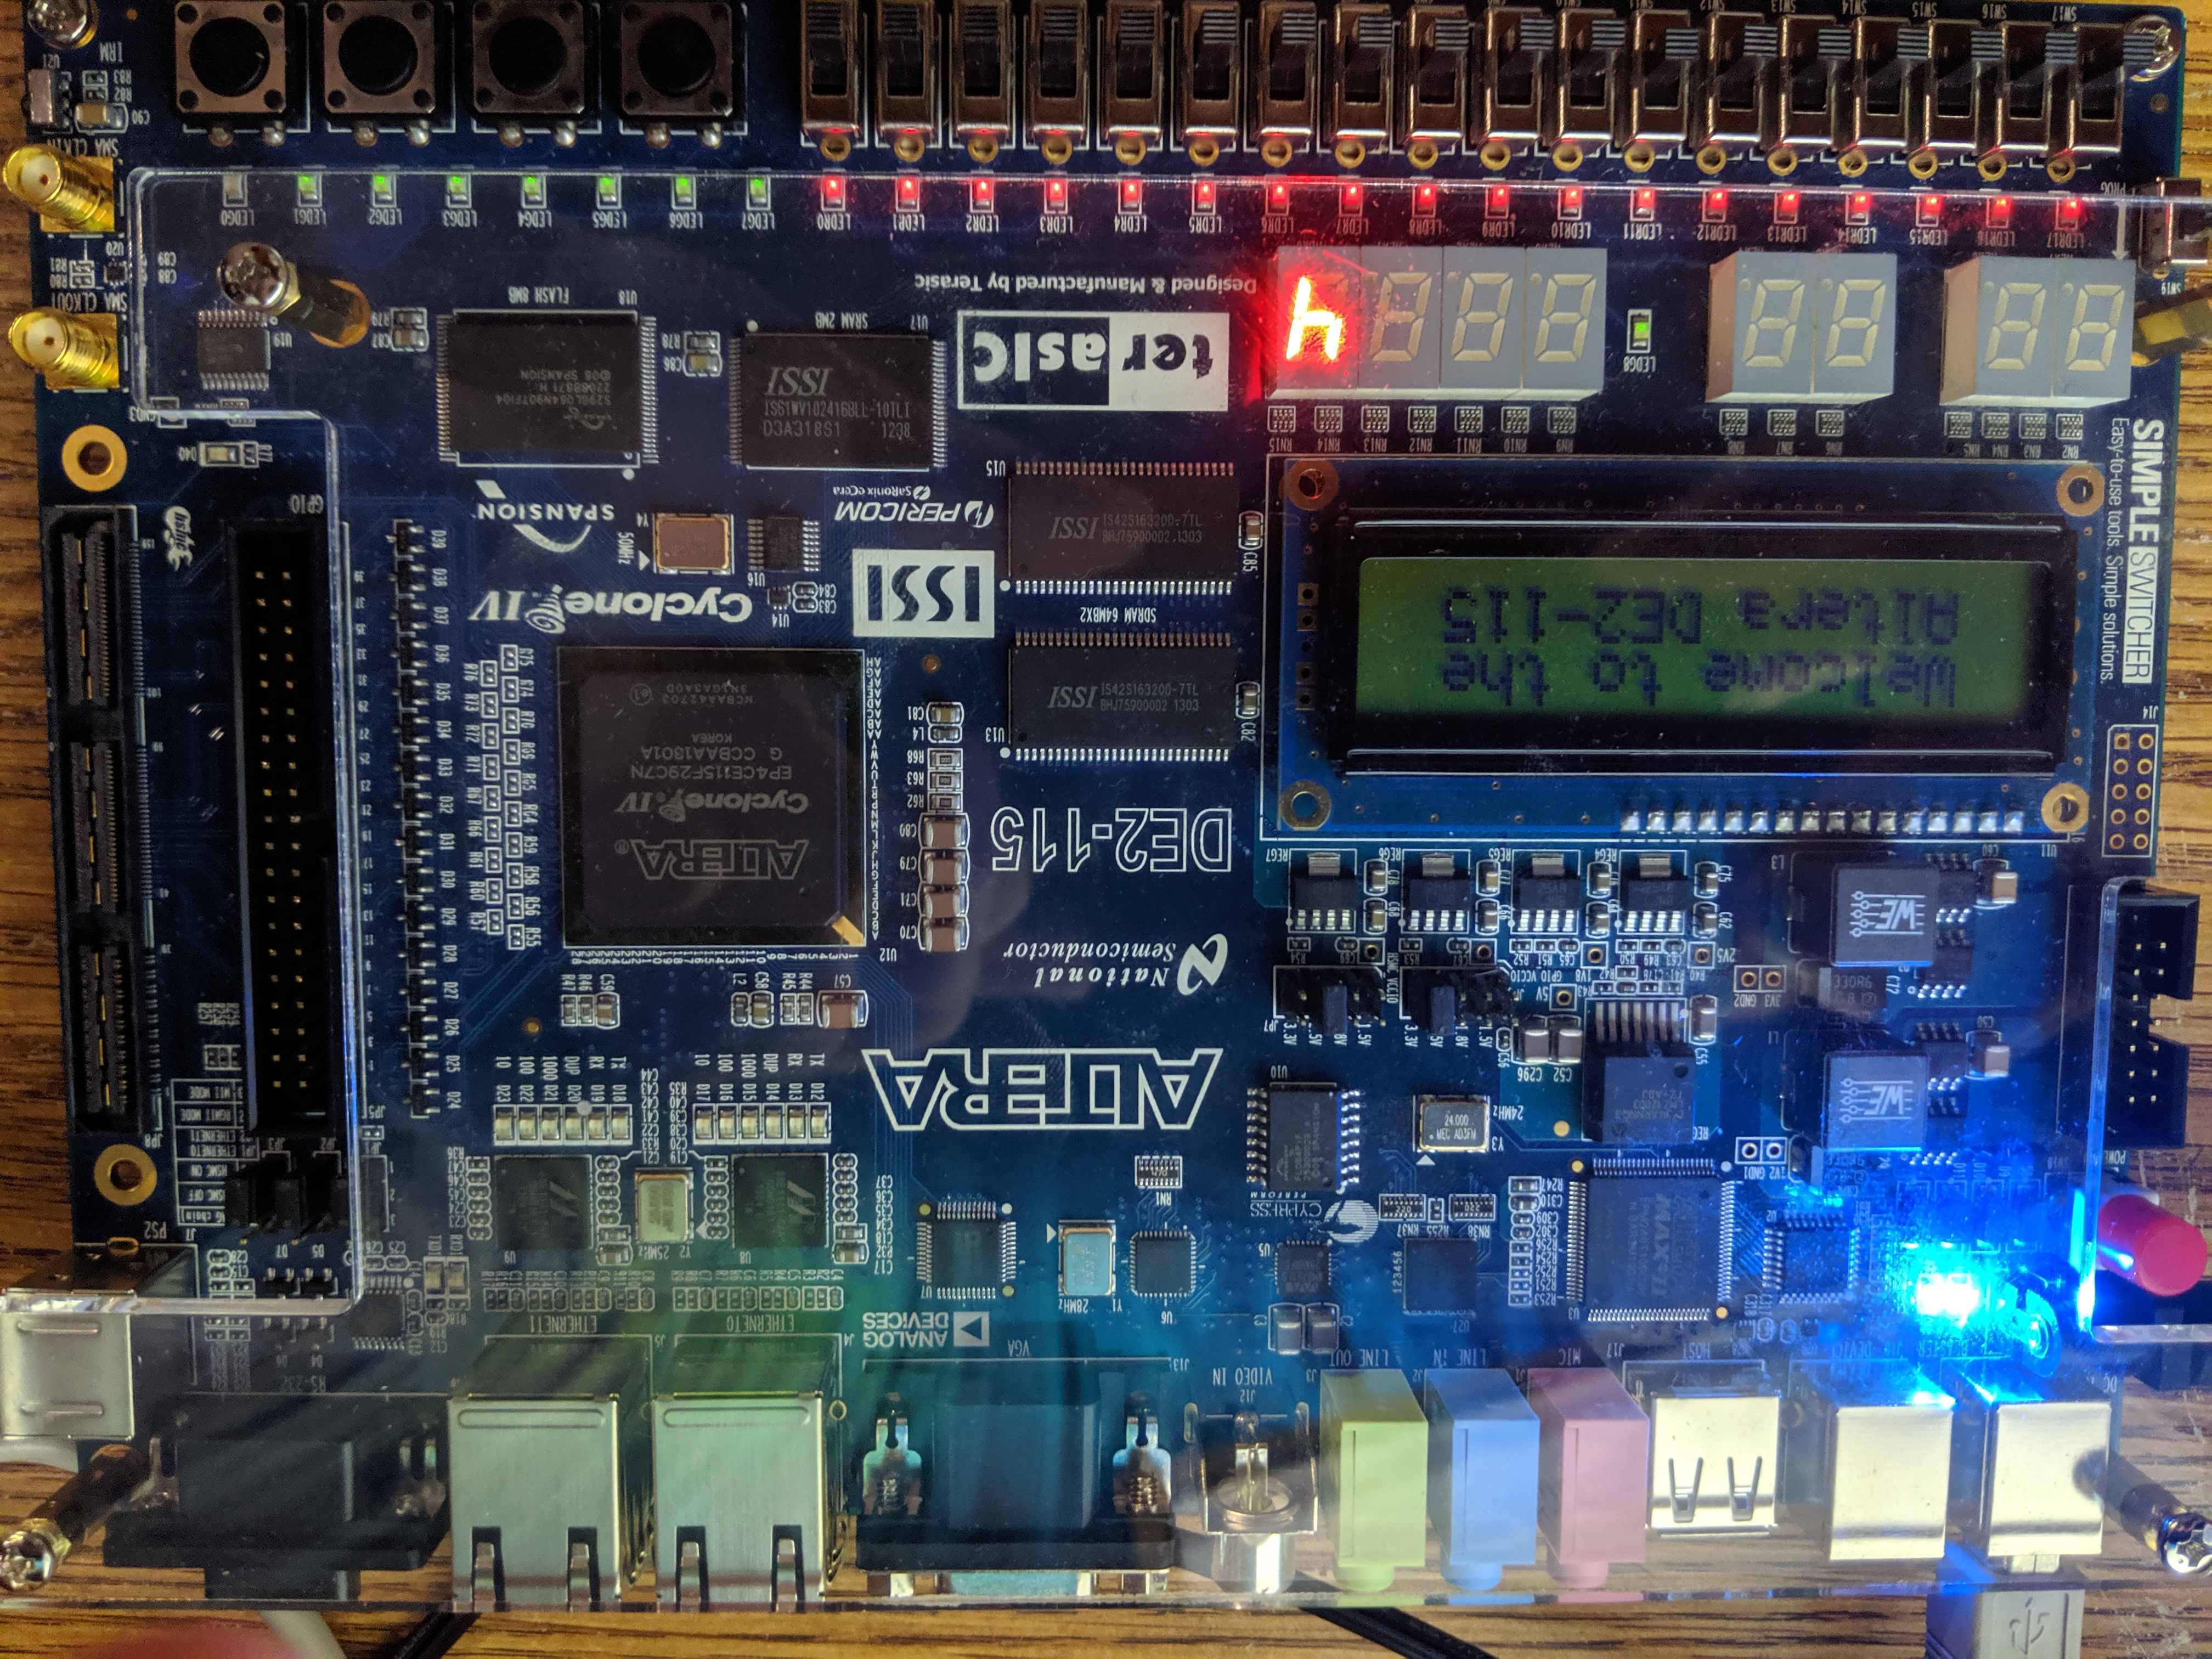
\includegraphics[width=3cm]{Display4.jpg}}
				\caption{Display 4}
			\end{subfigure}	
			\begin{subfigure}{3cm}
				\rotatebox[origin=c]{180}{\centering\includegraphics[width=3cm]{Display5.jpg}}
				\caption{Display 5}
			\end{subfigure}		
		
			\begin{subfigure}{3cm}
				\rotatebox[origin=c]{180}{\centering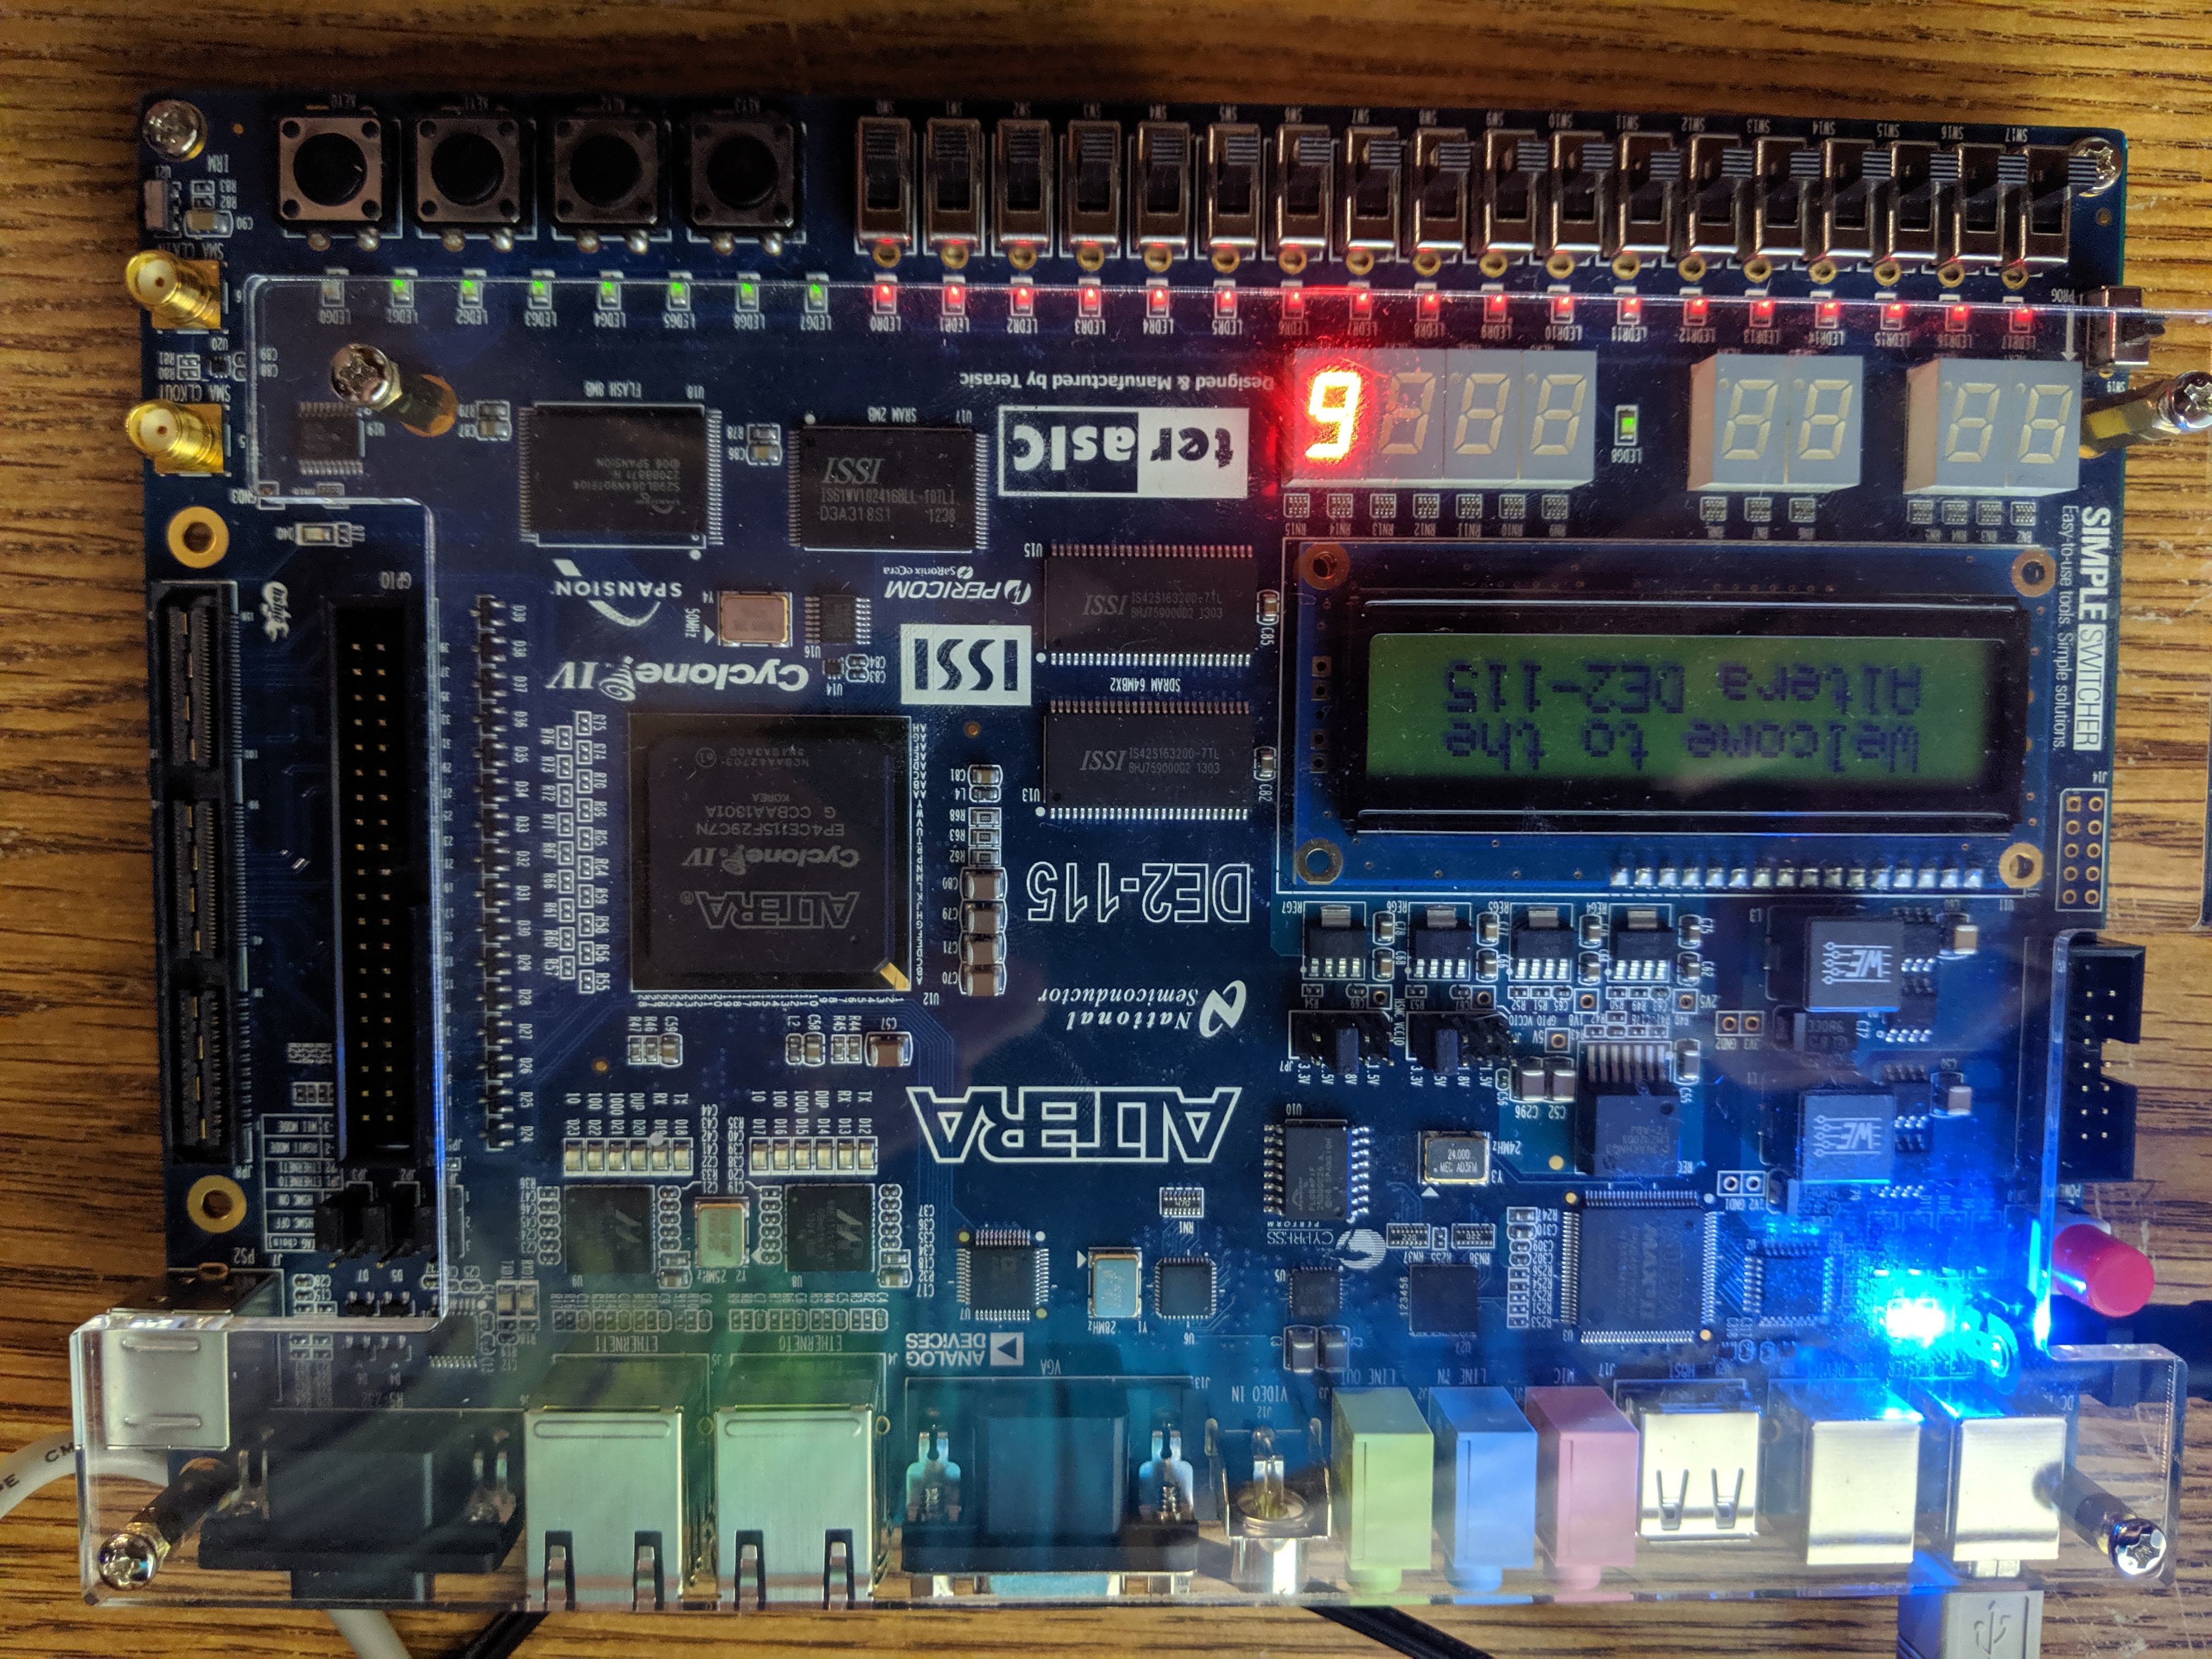
\includegraphics[width=3cm]{Display6.jpg}}
				\caption{Display 6}
			\end{subfigure}	
			\begin{subfigure}{3cm}
				\rotatebox[origin=c]{180}{\centering\includegraphics[width=3cm]{Display7.jpg}}
				\caption{Display 7}
			\end{subfigure}	
			\begin{subfigure}{3cm}
				\rotatebox[origin=c]{180}{\centering\includegraphics[width=3cm]{Display8.jpg}}
				\caption{Display 8}
			\end{subfigure}
		
			\begin{subfigure}{3cm}
				\rotatebox[origin=c]{180}{\centering\includegraphics[width=3cm]{Display9.jpg}}
				\caption{Display 9}
			\end{subfigure}					
		\label{fig:disp}
	\end{figure}
	\subsection{Button Polling}
	\begin{figure}[H]
		\rotatebox[origin=c]{90}{\includegraphics[height=15cm]{Polling.png}}
		\caption{Button Polling Results}
		\label{fig:polling}
	\end{figure}
	\appendix
	\section{\\VHDL Code}
	\lstinputlisting[language=VHDL]{homework1.vhd}
	
	\section{\\C Code}
	\subsection{Headers}
	\lstinputlisting[language=C]{counter.h}
	
	\subsection{Source}
	\lstinputlisting[language=C]{main.c}
	
	
\end{document}